% gc-04-ProductQuotient.tex

\documentclass[xcolor=dvipsnames]{beamer}
\usepackage{teachbeamer}

\title{Product and Quotient Rule}
\subtitle{{\CourseNumber}, BCIT}

\author{\CourseName}

\date{January 16, 2018}

% \begin{figure}[h]
% 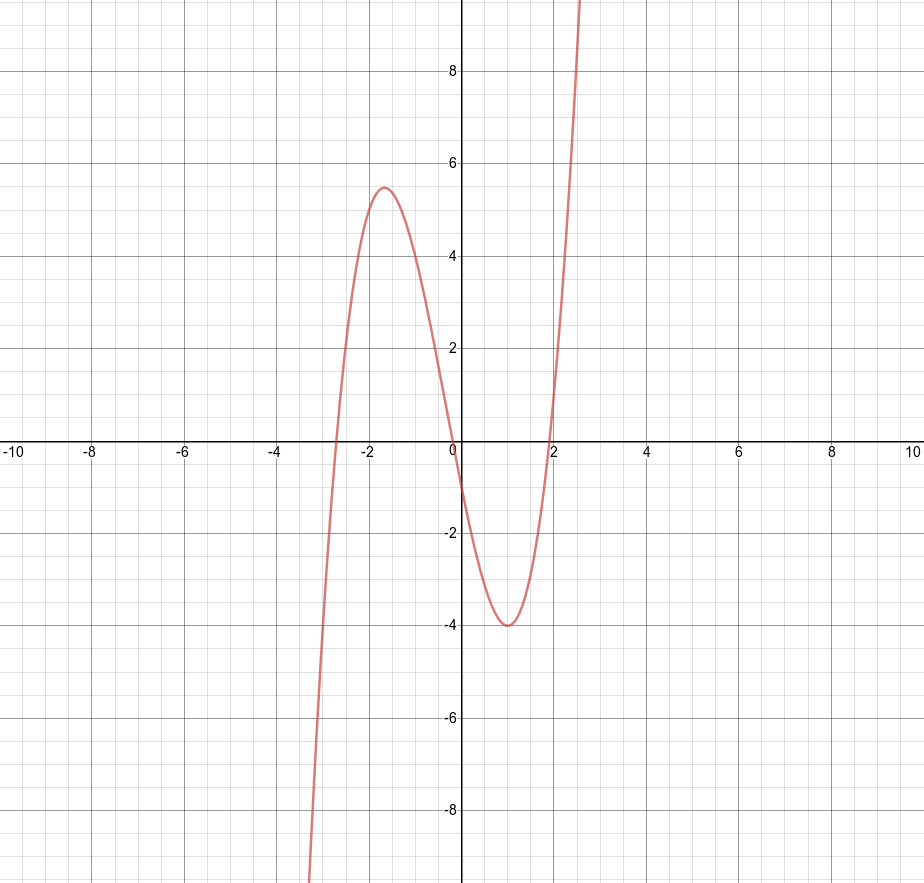
\includegraphics[scale=.3]{./diagrams/extrema1.png}
% \end{figure}

\begin{document}

\begin{frame}
  \titlepage
\end{frame}

\begin{frame}
  \frametitle{Product Rule}
  \begin{block}{Rule 5}
The Product Rule
  \end{block}
\begin{equation}
  \label{eq:aepuaxai}
g'(x)=f_{1}(x)f_{2}'(x)+f_{1}'(x)f_{2}(x)\mbox{ for }g(x)=f_{1}(x)f_{2}(x)
\end{equation}
\end{frame}

\begin{frame}
  \frametitle{Product Rule Reason}
Reason:
\begin{equation}
  \label{eq:yahtiera}
g'(x)=\notag
\end{equation}
\begin{equation}
  \label{eq:piebaith}
\lim_{h\rightarrow{}0}\frac{g(x+h)-g(x)}{h}=\lim_{h\rightarrow{}0}\frac{f_{1}(x+h)f_{2}(x+h)-f_{1}(x)f_{2}(x)}{h}=\notag
\end{equation}
\begin{equation}
  \label{eq:eceishie}
\lim_{h\rightarrow{}0}\frac{f_{1}(x+h)f_{2}(x+h)\alert{-f_{1}(x)f_{2}(x+h)+f_{1}(x)f_{2}(x+h)}-f_{1}(x)f_{2}(x)}{h}=\notag
\end{equation}
\begin{equation}
  \label{eq:chiekeey}
\lim_{h\rightarrow{}0}\frac{(f_{1}(x+h)-f_{1}(x))f_{2}(x+h)+f_{1}(x)(f_{2}(x+h)-f_{2}(x))}{h}=\notag
\end{equation}
\begin{equation}
  \label{eq:vaeyiewe}
f_{1}(x)f_{2}'(x)+f_{1}'(x)f_{2}(x)
\end{equation}
\end{frame}

\begin{frame}
  \frametitle{Product Rule Exercises}
Differentiate the following functions.
\begin{equation}
  \label{eq:iefeiwah}
f(x)=(2x^{2}-1)(x^{3}+3)
\end{equation}
\begin{equation}
  \label{eq:recootie}
g(t)=t^{3}\left(\sqrt{t}+1\right)
\end{equation}
\end{frame}

\begin{frame}
  \frametitle{Quotient Rule}
  \begin{block}{Rule 6}
The Quotient Rule
  \end{block}
\begin{equation}
  \label{eq:roothubu}
g'(x)=\frac{f_{1}'(x)f_{2}(x)-f_{1}(x)f_{2}'(x)}{\left(f_{2}(x)\right)^{2}}\mbox{ for }g(x)=\frac{f_{1}(x)}{f_{2}(x)}
\end{equation}
\end{frame}

\begin{frame}
  \frametitle{Quotient Rule Reason}
Reason:
\begin{equation}
  \label{eq:iebowohc}
g(x)=\frac{f_{1}(x)}{f_{2}(x)}
\end{equation}
\begin{equation}
  \label{eq:iilahthi}
f_{1}(x)=g(x)f_{2}(x)
\end{equation}
\begin{equation}
  \label{eq:eshohhoo}
f_{1}'(x)=g'(x)f_{2}(x)+g(x)f_{2}'(x)\mbox{ now isolate }g'(x)
\end{equation}
\begin{equation}
  \label{eq:iophiewu}
g'(x)=\frac{f_{1}'(x)-g(x)f_{2}'(x)}{f_{2}(x)}\mbox{ now substitute }g(x)=\frac{f_{1}(x)}{f_{2}(x)}
\end{equation}
\begin{equation}
  \label{eq:uhushain}
g'(x)=\frac{\frac{f_{1}'(x)f_{2}(x)}{f_{2}(x)}-\frac{f_{1}(x)f_{2}'(x)}{f_{2}(x)}}{f_{2}(x)}
\end{equation}
\begin{equation}
  \label{eq:requuare}
g'(x)=\frac{f_{1}'(x)f_{2}(x)-f_{1}(x)f_{2}'(x)}{\left(f_{2}(x)\right)^{2}}
\end{equation}
\end{frame}

\begin{frame}
  \frametitle{Quotient Rule Exercises}
Differentiate the following functions.
\begin{equation}
  \label{eq:xookaeji}
f(z)=\frac{3z^{2}+5z-2}{3z-1}
\end{equation}
\begin{equation}
  \label{eq:eidoogow}
h(x)=\frac{\sqrt{x}}{x^{2}+1}
\end{equation}
\end{frame}

\begin{frame}
  \frametitle{Quotient Rule Exercise Solution}
  \begin{figure}[h]
    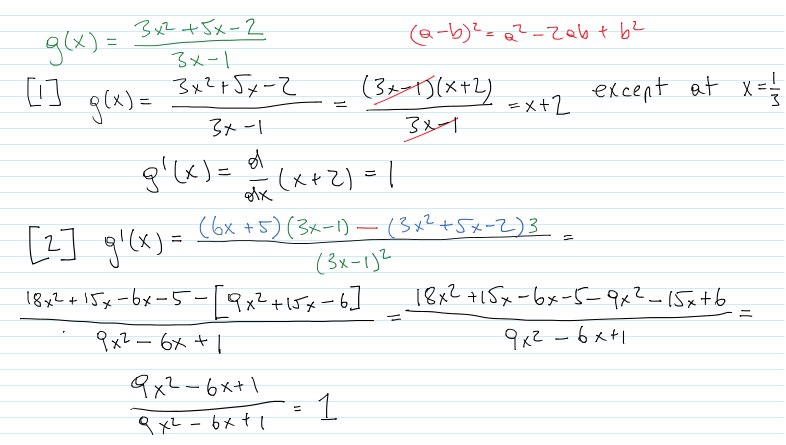
\includegraphics[scale=0.575]{./diagrams/onenote_ft_09_ProductQuotientRule_02.png}
  \end{figure}
\end{frame}

\begin{frame}
  \frametitle{End of Lesson}
Next Lesson: Chain Rule
\end{frame}

\end{document}
